\documentclass[aspectratio=169]{beamer}
\usepackage[utf8]{inputenc}
\usepackage{amsmath}
\usepackage{tikz}
\usepackage{dsfont}
\usepackage{opensans}

\usetheme{NOVASBE}

\title[]{4509 - Bridging Mathematics}
\subtitle{Vectors}
\author[P. Fagandini]{Paulo Fagandini}
\institute{}
\date{}

\newtheorem{defenition}{Definition}[section]
\newtheorem{proposition}{Conjecture}[section]

\begin{document}

\begin{frame}{Notation}
    Notation is important. For this set of slides consider:
    \begin{enumerate}
        \item Lowercase for elements of a \emph{vector}, $v_i$.
        \item Uppercase for vectors/matrices, $V$.
        \item Calligraphic uppercase for sets, e.g., set $\mathcal{S}$.
    \end{enumerate}
\end{frame}


\begin{frame}
    \begin{center}
        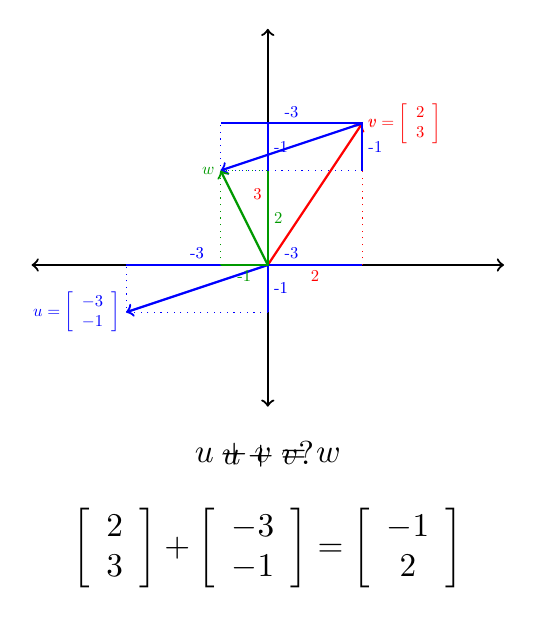
\begin{tikzpicture}[scale=0.6,every node/.style = {scale = 0.6}]
            \draw[<->,thick] (-5,0) -- (5,0);
            \draw[<->,thick] (0,-3) -- (0,5);

            \onslide<2->{
                \draw[thick,red,->] (0,0) -- (2,3);
            }

            \onslide<2-4>{
                \draw[red](2,3) node[right]{$v$};
            }

            \onslide<3-11>{
                \draw[red,thick] (0,0) -- (2,0)node[midway,below]{2};
                \draw[red,dotted] (2,0) -- (2,3);
            }
            \onslide<4-11>{
                \draw[red,thick] (0,0) -- (0,3)node[midway,left]{3};
                \draw[red,dotted] (0,3) -- (2,3);
            }

            \onslide<5-6>{
                \draw[red](2,3) node[right]{$v=\left[\begin{array}{c}2 \\ 3 \end{array}\right]$};
            }

            \onslide<6-7>{
                \draw[blue,thick,->] (0,0) -- (-3,-1);
                \draw[blue,thick] (0,-1) -- (0,0)node[midway,right]{-1} -- (-3,0) node[midway,above]{-3};
                \draw[blue,dotted] (0,-1) -- (-3,-1) -- (-3,0);
            }

            \onslide<6>{
                \draw[blue] (-3,-1)node[left]{$u = \left[\begin{array}{c}-3 \\ -1 \end{array}\right]$};
            }

            \onslide<7>{
                \draw[](0,-4)node[scale=2]{$u+v?$};
            }

            \onslide<8-10>{
                \draw[blue,thick,->,opacity=0.3] (0,0) -- (-3,-1);
                \draw[blue,thick,opacity=0.3] (0,-1) -- (0,0)node[midway,right]{-1} -- (-3,0) node[midway,above]{-3};
                \draw[blue,dotted,opacity=0.3] (0,-1) -- (-3,-1) -- (-3,0);
            }

            \onslide<9->{
                \draw[blue,thick,->] (2,3) -- (-1,2);
            }

            \onslide<9>{
                \draw[blue,thick] (2,2) -- (2,3)node[midway,right]{-1} -- (-1,3) node[midway,above]{-3};
                \draw[blue,dotted] (2,2) -- (-1,2) -- (-1,3);   
            }

            \onslide<10-11>{
                \draw[blue,thick] (0,2) -- (0,3)node[midway,right]{-1};
                \draw[blue,thick] (2,0) -- (-1,0) node[midway,above]{-3};

            }

            \onslide<11->{
                \draw[green!60!black,thick] (-1,0) -- (0,0) node[below,midway]{-1} -- (0,2)node[right,midway]{2};
            }

            \onslide<12->{
                \draw[green!60!black,thick,->] (0,0) -- (-1,2)node[left]{$w$};
                \draw[green!60!black,dotted] (-1,0) -- (-1,2) -- (0,2);
            }

            \onslide<13->{
                \draw[](0,-4)node[scale=2]{$u+v=w$};
            }

            \onslide<14->{
                \draw[](0,-6)node[scale=2]{$\left[\begin{array}{c}2\\3\end{array}\right]+\left[\begin{array}{c}-3\\-1\end{array}\right]=\left[\begin{array}{c}-1\\2\end{array}\right]$};
            }

        \end{tikzpicture}
    \end{center}
\end{frame}

\begin{frame}
    \begin{center}
        \begin{tikzpicture}[scale=0.6,every node/.style = {scale = 0.6}]
            \draw[<->,thick] (-5,0) -- (5,0);
            \draw[<->,thick] (0,-3) -- (0,5);

            \onslide<2-3>{
                \draw[thick,red,->] (0,0) -- (2,3);
                \draw[red](2,3) node[right]{$v=\left[\begin{array}{c}2 \\ 3 \end{array}\right]$};
                \draw[red,thick] (0,0) -- (2,0)node[midway,below]{2};
                \draw[red,thick] (0,0) -- (0,3)node[midway,left]{3};
            }

            \onslide<4->{
                \draw[thick,red,->,opacity=0.2] (0,0) -- (2,3);
                \draw[red,opacity=0.2](2,3) node[right]{$v=\left[\begin{array}{c}2 \\ 3 \end{array}\right]$};
                \draw[red,thick,opacity=0.2] (0,0) -- (2,0)node[midway,below]{2};
                \draw[red,thick,opacity=0.2] (0,0) -- (0,3)node[midway,left]{3};
            }

            \onslide<3>{
                \draw[](0,-6)node[scale=2]{$0.5 v ?$};
            }

            \onslide<4>{
                \draw[red,thick,->] (0,0) -- (1,1.5)node[right]{$0.5v=\left[\begin{array}{c}1 \\ 1.5 \end{array}\right]$};
                \draw[red,thick] (0,0) -- (1,0)node[midway,below]{1};
                \draw[red,thick] (0,0) -- (0,1.5)node[midway,left]{1.5};
            }

            \onslide<5->{
                \draw[red,thick,->,opacity=0.2] (0,0) -- (1,1.5)node[right]{$0.5v=\left[\begin{array}{c}1 \\ 1.5 \end{array}\right]$};
                \draw[red,thick,opacity=0.2] (0,0) -- (1,0)node[midway,below]{1};
                \draw[red,thick,opacity=0.2] (0,0) -- (0,1.5)node[midway,left]{1.5};
            }

            \onslide<5>{
                \draw[red,thick,->] (0,0) -- (3,4.5)node[right]{$1.5v=\left[\begin{array}{c}3 \\ 4.5 \end{array}\right]$};
                \draw[red,thick] (0,0) -- (3,0)node[midway,below]{3};
                \draw[red,thick] (0,0) -- (0,4.5)node[midway,left]{4.5};
            }

            \onslide<6>{
                \draw[red,thick,->,opacity=0.2] (0,0) -- (3,4.5)node[right]{$1.5v=\left[\begin{array}{c}3 \\ 4.5 \end{array}\right]$};
                \draw[red,thick,opacity=0.2] (0,0) -- (3,0)node[midway,below]{3};
                \draw[red,thick,opacity=0.2] (0,0) -- (0,4.5)node[midway,left]{4.5};
            }

            \onslide<6>{
                \draw[red,thick,->] (0,0) -- (-2,-3)node[left]{$-1 v=\left[\begin{array}{c}-2 \\ -3 \end{array}\right]$};
                \draw[red,thick] (0,0) -- (-2,0)node[midway,above]{-2};
                \draw[red,thick] (0,0) -- (0,-3)node[midway,right]{-3};
            }


        \end{tikzpicture}
    \end{center}
\end{frame}

\begin{frame}
    \begin{center}
        \begin{tikzpicture}[scale=0.6,every node/.style = {scale = 0.6}]
            \draw[<->,thick] (-5,0) -- (5,0);
            \draw[<->,thick] (0,-3) -- (0,5);
            \def\vx{2}
            \def\vy{3}
            \def\ux{-3}
            \def\uy{-1}
            \def\a{-1/2}
            \def\b{-3/4}

            \onslide<1>{
                \draw[red,->,thick] (0,0) -- (\vx,\vy)node[right]{$v$};
                \draw[blue,->,thick] (0,0) -- (\ux,\uy)node[left]{$u$};
            }

            \onslide<2->{
                \draw[red,->,thick, opacity = 0.2] (0,0) -- (\vx,\vy)node[right]{$v$};
                \draw[blue,->,thick, opacity = 0.2] (0,0) -- (\ux,\uy)node[left]{$u$};
            }

            \onslide<2->{
                \draw[orange,->,thick] (0,0) -- ({\a*\vx+\b*\ux},{\a*\vy+\b*\uy})node[right]{$z$};
            }

            \onslide<3->{
                \draw[red,->,thick] (0,0) -- ({\a*\vx},{\a*\vy})node[left]{$\a\times v$};
            }
            \onslide<4>{
                \draw[blue,->,thick] (0,0) -- ({\b*\ux},{\b*\uy})node[right]{$\b\times u$};
            }

            \onslide<5->{
                \draw[blue,->,thick,dotted] (0,0) -- ({\b*\ux},{\b*\uy})node[right]{$\b\times u$};
                \draw[blue,->,thick] ({\a*\vx},{\a*\vy}) -- ({\a*\vx+\b*\ux},{\a*\vy+\b*\uy});
            }

            \onslide<6>{
                \draw[] (1,-3)node[right,scale=2]{$z=\a\times v + \b\times u$};
            }

        \end{tikzpicture}
    \end{center}
\end{frame}

\begin{frame}
    \begin{center}
        \begin{tikzpicture}[scale=0.6,every node/.style = {scale = 0.6}]
            \draw[<->,thick] (-5,0) -- (5,0);
            \draw[<->,thick] (0,-3) -- (0,5);
            \def\vx{2}
            \def\vy{3}
            \def\ux{-3}
            \def\uy{-1}
            \def\a{1/4}
            \def\b{-3/5}

            \onslide<1->{
                \draw[red,->,thick, opacity = 0.2] (0,0) -- (\vx,\vy)node[right]{$v$};
                \draw[blue,->,thick, opacity = 0.2] (0,0) -- (\ux,\uy)node[left]{$u$};
                \draw[orange,->,thick] (0,0) -- ({\a*\vx+\b*\ux},{\a*\vy+\b*\uy})node[right]{$z$};
            }
            \onslide<2->{
                \draw[red,->,thick] (0,0) -- ({\a*\vx},{\a*\vy})node[left]{$\a\times v$};
                \draw[blue,->,thick,dotted] (0,0) -- ({\b*\ux},{\b*\uy})node[right]{$\b\times u$};
                \draw[blue,->,thick] ({\a*\vx},{\a*\vy}) -- ({\a*\vx+\b*\ux},{\a*\vy+\b*\uy});
                \draw[] (1,-3)node[right,scale=2]{$z=\a\times v + \b\times u$};
            }

        \end{tikzpicture}
    \end{center}
\end{frame}

\begin{frame}
    \begin{center}
        \begin{tikzpicture}[scale=0.6,every node/.style = {scale = 0.6}]
            \draw[<->,thick] (-5,0) -- (5,0);
            \draw[<->,thick] (0,-3) -- (0,5);
            \def\vx{2}
            \def\vy{3}
            \def\ux{-3}
            \def\uy{-1}
            \def\a{1/3}
            \def\b{3/7}

            \onslide<1->{
                \draw[red,->,thick, opacity = 0.2] (0,0) -- (\vx,\vy)node[right]{$v$};
                \draw[blue,->,thick, opacity = 0.2] (0,0) -- (\ux,\uy)node[left]{$u$};
                \draw[orange,->,thick] (0,0) -- ({\a*\vx+\b*\ux},{\a*\vy+\b*\uy})node[right]{$z$};
            }
            \onslide<2->{
                \draw[red,->,thick] (0,0) -- ({\a*\vx},{\a*\vy})node[left]{$\a\times v$};
                \draw[blue,->,thick,dotted] (0,0) -- ({\b*\ux},{\b*\uy})node[left]{$\b\times u$};
                \draw[blue,->,thick] ({\a*\vx},{\a*\vy}) -- ({\a*\vx+\b*\ux},{\a*\vy+\b*\uy});
                \draw[] (1,-3)node[right,scale=2]{$z=\a\times v + \b\times u$};
            }
        \end{tikzpicture}
    \end{center}
\end{frame}

\begin{frame}
    We can write any vector in the plane as the result of the product and sum of $u$ and $v$ (a.k.a. a \emph{linear combination}). These vectors, are not special, except for 1 thing... they are linearly independent.
\end{frame}

\begin{frame}
    Consider now these two vectors {\color{red}$e$} and {\color{blue}$f$}...
    \begin{center}
        \begin{tikzpicture}[scale=0.6,every node/.style = {scale = 0.6}]
            \draw[<->,thick] (-5,0) -- (5,0);
            \draw[<->,thick] (0,-3) -- (0,5);
            \def\vx{3}
            \def\vy{2}
            \def\a{1/3}

            \def\b{0.7}
            \def\c{-0.2}

            \onslide<1>{
                \draw[red,->,thick] (0,0) -- (\vx,\vy)node[right]{$e$};
                \draw[blue,->,thick] (0,0) -- (\a*\vx,\a*\vy)node[right]{$f$};
            }

            \onslide<2->{
                \draw[red,->,thick,opacity=0.2] (0,0) -- (\vx,\vy)node[right]{$e$};
                \draw[blue,->,thick,opacity=0.2] (0,0) -- (\a*\vx,\a*\vy)node[right]{$f$};

                \draw[orange,->,thick] (0,0) -- ({\b*\vx+\a*\c*\vx},{\b*\vy+\a*\c*\vy})node[right,color=black]{$d=\b\times e+\c\times f$};
            }

        \end{tikzpicture}
    \end{center}
\end{frame}

\begin{frame}
    Consider now these two vectors {\color{red}$e$} and {\color{blue}$f$}...
    \begin{center}
        \begin{tikzpicture}[scale=0.6,every node/.style = {scale = 0.6}]
            \draw[<->,thick] (-5,0) -- (5,0);
            \draw[<->,thick] (0,-3) -- (0,5);
            \def\vx{3}
            \def\vy{2}
            \def\a{1/3}

            \def\b{-0.7}
            \def\c{-0.3}

            \draw[red,->,thick,opacity=0.2] (0,0) -- (\vx,\vy)node[right]{$e$};
            \draw[blue,->,thick,opacity=0.2] (0,0) -- (\a*\vx,\a*\vy)node[right]{$f$};

            \draw[orange,->,thick] (0,0) -- ({\b*\vx+\a*\c*\vx},{\b*\vy+\a*\c*\vy})node[right,color=black]{$d=\b\times e+\c\times f$};

        \end{tikzpicture}
    \end{center}
\end{frame}

\begin{frame}
    We can only ``create'' vectors along the same line, the line that goes in the direction of vectors $e$ and $f$. These vectors are linearly dependent.
    
    \vspace{0.3cm}

    Actually, we only needed one of them to create all the others that we could draw!

\end{frame}

\begin{frame}
    \begin{center}
        \begin{tikzpicture}[scale=0.6,every node/.style = {scale = 0.6}]
            \draw[<->,thick] (-5,0) -- (5,0);
            \draw[<->,thick] (0,-3) -- (0,5);
            \def\vx{3}
            \def\vy{2}

            \draw[red,->,thick,] (0,0) -- (\vx,\vy)node[right]{$v$};
            
            \onslide<2->{
                \draw[red,->,thick] (0,0) -- (\vx,0)node[below,midway]{$\vx$};
                \draw[red,->,thick] (0,0) -- (0,\vy)node[left,midway]{$\vy$};
            }

            \onslide<3->{
                \draw[blue,->,thick] (0,0) -- (1,0)node[below,midway]{$\hat{\imath}$};
                \draw[blue,->,thick] (0,0) -- (0,1)node[left,midway]{$\hat{\jmath}$};
            }

            \onslide<4->{
                \draw[] (1,-1) node[right]{$v=3\times\hat{\imath}+2\times\hat{\jmath}=3\times\underbrace{\left[\begin{array}{c}1\\0\end{array}\right]}_{\hat{\imath}}+2\times\underbrace{\left[\begin{array}{c}0\\1\end{array}\right]}_{\hat{\jmath}}=\left[\begin{array}{c}3\\2\end{array}\right]$};
            }

        \end{tikzpicture}
    \end{center}   
\end{frame}

\begin{frame}
    \begin{definition}
        A \textbf{vector} is an element $V$ of $\mathds{R}^n$, for $n\geq 2$. A scalar is an element of $\mathds{R}$.
    \end{definition}
    
    Vectors are to be written as columns, example:
    
    \begin{align*}
        V=\left(\begin{array}{c}
             v_1  \\
             v_2\\
             \hdots \\
             v_{n-1}\\
             v_n
        \end{array}\right) \quad \in \quad \mathds{R}^n
    \end{align*}
\end{frame}

\begin{frame}

    Let $X,Y\in\mathds{R}^n$, and $\alpha\in\mathds{R}$, then
    
    \begin{enumerate}
        \item The sum,
        
        \begin{align*}
            X+Y&=\left(\begin{array}{c} x_1\\ \vdots \\x_n\end{array}\right)+\left(\begin{array}{c}y_1\\ \vdots\\ y_n\end{array}\right)=\left(\begin{array}{c}x_1+y_1\\ \vdots \\ x_n+y_n\end{array}\right)
    \end{align*}
    
        \item Scalar multiplication,
        
        \begin{align*}
            \alpha X &= \left(\begin{array}{c}\alpha x_1\\ \vdots \\ \alpha x_n\end{array}\right)
        \end{align*}
        
    \end{enumerate}

\end{frame}

\begin{frame}
    $0\in\mathds{R}^n$ is,
    
    \begin{align*}\left(
        \begin{array}{c}
            0\\
            \vdots\\
            0
        \end{array}\right)
    \end{align*} that is a vector of dimension $n\times 1$ filled with zeroes.
\end{frame}

\begin{frame}
    \begin{definition}
        A \textbf{vector space} $\mathcal{S}$, satisfies that, for any $A,B \in \mathcal{S}$, and $\alpha\in \mathds{R}$,
        
        \begin{itemize}
            \item $(A+B)\in \mathcal{S}$
            \item $\alpha A \in \mathcal{S}$
        \end{itemize}
    \end{definition}
    
    It is trivial to show that $\mathds{R}^n$ is a vector space.
    
    \begin{definition}
        A nonempty set $\mathcal{S}\subseteq \mathds{R}^n$ is a \textbf{vector subspace} of $\mathds{R}^n$ if, with the vector addition and the scalar multiplication it is a vector space by itself.
    \end{definition}
\end{frame}

\begin{frame}
    \begin{proposition}
       Let $\mathcal{V}\subseteq\mathds{R}^n$, nonempty. $\mathcal{V}$ is a vector subspace of $\mathds{R}^n$ if and only if,
        
        \begin{enumerate}
            \item $0\in \mathcal{V}$,
            \item $a,b\in \mathcal{V}$, $\alpha\in \mathds{R}$, then $a+\alpha b\in \mathcal{V}$
        \end{enumerate}
    \end{proposition}
    
    \pause
    
    Quick quiz! 15 min to prove it!
    
\end{frame}

\begin{frame}
    \begin{proof}
        \begin{itemize}
            \item $\Rightarrow$... If $\mathcal{V}$ is v.s. of $\mathds{R}^n$, we know that the scalar multiplication and the sum is in the space. Because scalar mult. we know that $\alpha b\in\mathcal{V}$, so the sum must be in $\mathcal{V}$ too. \pause
            
            \item $\Leftarrow$... If $a+\alpha b \in\mathcal{V}$, then it holds in  particular for $\alpha = 1$, so the sum is \emph{closed} in the space. Also, let $a = 0$, and you have the scalar multiplication. Then $\mathcal{V}$ must be a v.s.
        \end{itemize}
    \end{proof}
\end{frame}

\begin{frame}
    
    \begin{definition}

    Let $\mathcal{V}\subseteq\mathds{R}^n$ be a set of $k$ vectors, then, $Z\in\mathds{R}^n$ is a \textbf{linear combination} of the vectors $\{V_i\}_{i=1}^k$in $\mathcal{V}$ if there are scalars $\alpha_j$ $j=1,...,k$ such that,
    
    \begin{align*}
        Z = \sum_{j=1}^k \alpha_j V_j  
    \end{align*}
    
    \end{definition}
    
    \begin{definition}
        A \textbf{linear subspace} generated by the vectors in $\mathcal{V}$, represented $L(\mathcal{V})$, is the set of all the linear combinations of those vectors.
    \end{definition}
\end{frame}

\begin{frame}
    \begin{proposition}
        \begin{enumerate}
            \item Let $\mathcal{V},\mathcal{W}\subseteq\mathds{R}^n$, such that $\mathcal{V}\subseteq \mathcal{W}$, then $L(\mathcal{V})\subseteq L(\mathcal{W})$
            \item If $Y\in L(\mathcal{V})$, then $L(\{Y\}\cup \mathcal{V}) = L(\mathcal{V})$
            \item Given a nonempty $\mathcal{V}\subseteq\mathds{R}^n$, then $L(\mathcal{V})$ is a vector subspace of $\mathds{R}^n$.
        \end{enumerate}\pause
    \end{proposition}
    
    Quick quiz! Prove it $\rightarrow$ 15 min.
    
\end{frame}

\begin{frame}
    \begin{proof}
    \begin{enumerate}
        \item Trivial. If $X\in L(\mathcal{V}) \Rightarrow X = \sum_{v_i\in\mathcal{V}} \alpha_i v_i$, and because $\mathcal{V}\subseteq\mathcal{W}$ those vectors are also part of $\mathcal{W}$, so $X\in L(\mathcal{W})$, so $L(\mathcal{V})\subseteq L(\mathcal{W})$.\pause
        \item \begin{itemize}
                \item As $\mathcal{V}\subseteq\mathcal{V}\cup \{Y\}$, we have that $L(\mathcal{V})\subseteq L(\mathcal{V}\cup \{Y\})$. \pause
                \item We need then $L(\mathcal{V}\cup \{Y\})\subseteq L(\mathcal{V})$.\pause
                \item Let $X\in L(\mathcal{V}\cup\{Y\})$, then there are scalars $\alpha_i$ such that $$X = \sum_{v_i\in\mathcal{V}} \alpha_i v_i + \beta Y$$ \pause
                \item As $Y\in L(\mathcal{V})$ there are scalars $\gamma_i$ such that $Y = \sum_{v_i\in\mathcal{V}} \gamma_i v_i$\pause
                \item $X = \sum_{v_i\in\mathcal{V}} \alpha_i v_i + \beta \left(\sum_{v_i\in\mathcal{V}} \gamma_i v_i\right) = \sum_{v_i\in\mathcal{V}} (\alpha_i+\beta\gamma_i) v_i$. But $\alpha+\beta\gamma$ is a scalar, so\pause
                \item $X\in L(\mathcal{V})$, proof is complete.\pause
            \end{itemize}
        
        \item $0$ belongs to any $L()$, as it is the case with scalars $=0$. Now, let $X,Y\in L(\mathcal{V})$ and $\gamma\in\mathds{R}$; $X+\gamma Y = \sum_{v_i\in\mathcal{V}}(\alpha_i+\gamma \beta_i) v_i$ if we write each vector as a linear comb. For the same argument used before, we complete the proof.
    \end{enumerate}
    \end{proof}
    
\end{frame}

\begin{frame}

    \begin{definition}
    A set of $k$ vectors $\mathcal{V}\subseteq \mathds{R}^n$ is \textbf{linearly independent} if, $\forall \alpha_j \in \mathds{R}$
    
    $$\sum_{j=1}^k \alpha_k V_j =0\quad\Leftrightarrow\quad \alpha_j=0$$
    \end{definition}
    
    \begin{definition}
        Conversely, if there are $\{\alpha_i\}_{i=1}^k$, with at least one $\alpha_k\neq0$, then they are \textbf{linearly dependent.}
    \end{definition}
    
\end{frame}

\begin{frame}

    \begin{definition}

    The set of vectors $\mathcal{X}\subseteq\mathcal{V}$ \textbf{generates} the vector subspace $\mathcal{V}\subseteq\mathds{R}^n$ if any $V\in\mathcal{V}$ can be written as a linear combination of the vectors in $\mathcal{X}$.
    
    \vspace{0.5cm}
    
    Moreover, if the vectors in $\mathcal{X}$ are linearly independent, then $\mathcal{X}$ is called a \textbf{basis} of $\mathcal{V}$.
    
    \end{definition}
    
\end{frame}

\begin{frame}
\begin{proposition}
    Let $\mathcal{X}=\{X_1,X_2,\ldots,X_k\}$ a basis of the vector subspace $\mathcal{V}\subseteq\mathds{R}^n$. Then, for any $V\in\mathcal{V}$, there are \textbf{unique} scalars $\{\alpha_i\}_{i=1}^k$ such that
    
    \begin{align*}
        V = \alpha_1 X_1+\alpha_2 X_2 + \ldots + \alpha_k X_k
    \end{align*}
\end{proposition}

\begin{proposition}
    Any set of $n$ linearly independent vectors $\mathcal{X}\subseteq\mathds{R}^n$, generates $\mathds{R}^n$
\end{proposition}

\end{frame}

\begin{frame}
    \begin{definition}
        The \textbf{dimension} of a vector space $\mathcal{V}$ is the maximum number of $l.i.$ vectors that generates it. This number coincides with the number of vectors in any basis of the space. It is denoted $dim(\mathcal{V})$.
    \end{definition}
\end{frame}

\begin{frame}
    \begin{definition}
        Given $X,Y\in\mathds{R}^n$, the \textbf{inner product} corresponds to:
        
        \begin{align*}
            X\cdot Y = \sum_{j=1}^n x_j y_j \quad\in \mathds{R}
        \end{align*}
    \end{definition}
    
    \begin{definition}
        The \textbf{Euclidean norm} of a vector $X\in\mathds{R}^n$ is:
        
        \begin{align*}
            ||X||=\sqrt{X\cdot X} = \sqrt{\sum_{j=1}^n x_j^2} \quad \in\mathds{R}
        \end{align*}
    \end{definition}
\end{frame}

\begin{frame}
    \begin{definition}
        For $X,Y\in\mathds{R}^n$, the \textbf{Euclidean distance} between them is defined as:
        
        \begin{align*}
            d(X,Y)=||X-Y||
        \end{align*}
    \end{definition}
\end{frame}

\begin{frame}
    \begin{definition}
        For $X,Y\in\mathds{R}^n$, both different from zero, the \textbf{angle} between them, denoted as $\angle(X,Y)$, is defined as the value that satisfies,
        
        \begin{align*}
            \cos(\angle(X,Y))=\frac{X\cdot Y}{||X||\cdot||Y||}\quad\in\quad[-1,1]
        \end{align*}
    \end{definition}

    \begin{definition}
        Two vectors $X,Y$ are \textbf{orthogonal}, if $\angle(X,Y)=90^{\circ}$, or equivalently, $X\cdot Y=0$. It is denoted as $X\perp Y$.
    \end{definition}

\end{frame}

\begin{frame}
    
    \begin{definition}

    Let $X\in\mathds{R}^n$. If $||X||=1$, $X$ is a \textbf{unit vector}.
    
    \end{definition}
    
    \begin{definition}
    
    Consider two vectors $X,Y\in\mathds{R}^n$, both different from zero. The \textbf{projection} of $Y$ over $X$ is defined as:
    
    \begin{align*}
        proj_X Y=Y \cdot \frac{X}{||X||}
    \end{align*}
    
    The \textbf{rejection}, is defined as:
    
    \begin{align*}
        rej_X Y=Y-proj_X Y
    \end{align*}
    
    The rejection is orthogonal to $X$.
    
    \end{definition}
\end{frame}

\begin{frame}

\begin{center}
    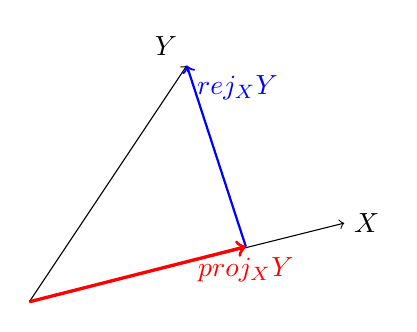
\begin{tikzpicture}
        \draw[->] (0,0) -- (4,1)node[anchor=west]{$X$};
        \draw[->] (0,0) -- (2,3)node[anchor= south east]{$Y$};
        
        \draw[blue,->,thick] (2.75,0.7)--(2,3) node[anchor=north west]{$rej_X Y$} ;
        
        \draw[red,->,very thick] (0,0) -- (2.75,0.7)node[anchor=north]{$proj_X Y$};
        
    \end{tikzpicture}
\end{center}

In econometrics, the endogenous variable would be $Y$. We try to explain it with the exogenous variable $X$, so we ``project'' $Y$ over $X$. Of course, what is not explained, the error, is $rej_X Y$.
    
\end{frame}

\begin{frame}

    \begin{definition}
        The \textbf{projection} of a vector $Y$ over a subspace $\mathcal{V}$ defined by a basis $\{X_1,X_2,\ldots,X_k\}$ is the vector $proj_\mathcal{V} Y$, and it must satisfy that
        
        \begin{align*}
            [proj_\mathcal{V} Y- Y]\perp X_i\quad \forall i=1,...,k
        \end{align*}
        
    \end{definition}
    
\end{frame}

\begin{frame}
    
    \begin{center}
    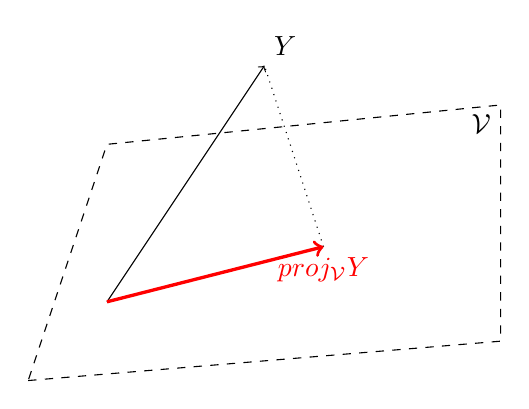
\begin{tikzpicture}
        
        \draw[dashed] (-1,-1) -- (5,-.5) -- (5,2.5)node[anchor=north east]{$\mathcal{V}$} -- (0,2) -- (-1,-1);
        
        \draw[->] (0,0) -- (2,3)node[anchor= south west]{$Y$};
        
        \draw[dotted] (2.75,0.7)--(2,3);
        
        \draw[red,->,very thick] (0,0) -- (2.75,0.7)node[anchor=north]{$proj_\mathcal{V} Y$};
        
    \end{tikzpicture}
    
    Here we could be projecting the exogenous variable over two explanatory variables...
    
\end{center}
    
\end{frame}

\end{document}
